\documentclass[12pt, french]{article}

\usepackage{fancyhdr, fancybox, lastpage}
\usepackage[most]{tcolorbox}
\usepackage[a4paper, margin={0.3in, .75in}]{geometry}
\usepackage{wrapfig}
\pagestyle{fancy}
\renewcommand\headrulewidth{1pt}
\renewcommand\footrulewidth{1pt}
\fancyhf{}
\rhead{ \em{Zakaria Haouzan}}
\lhead[C]{\em{1ére année baccalauréat Sciences Mathématiques}}
\chead[C]{}
\rfoot[C]{}
\lfoot[R]{}
\cfoot[]{\em{Page \thepage / \pageref{LastPage}}}


\newtcolorbox{Box2}[2][]{
                lower separated=false,
                colback=white,
colframe=white!20!black,fonttitle=\bfseries,
colbacktitle=white!30!gray,
coltitle=black,
enhanced,
attach boxed title to top left={yshift=-0.1in,xshift=0.15in},
title=#2,#1}


\begin{document}
\begin{center}
   \shadowbox {\bf{Énergie cinétique et travail }}
\end{center}


%%_________________________Exercice ! :"_________________________Exercice
   \begin{Box2}{Exercice 1 : }
Une machine tournante a une fréquence de rotation égale à 200 tr/min. Son moment d'inertie par rapport à son axe de rotation est égal à $50 kg. m^2$ . On prendra g = 10 N/ kg.
Pour l'arrêter on exerce une force tangentielle constante de 150 N.

1. Calculer la variation d'énergie cinétique au cours du freinage.

2.Calculer le moment de la force de freinage sachant que la machine peut être assimilée à un disque de diamètre $80 cm$.

3. Calculer le nombre de tours effectués par la machine avant l'arrêt.
   \end{Box2}


%%_________________________Exercice !2 :"_________________________Exercice
\begin{Box2}{Exercice 2 : }
Un volant est constitué d'un cylindre de fonte de masse M = 1 tonne entièrement répartie sur une circonférence de rayon R = 1 m. Il tourne à une vitesse de 300 tours par minute. .

1. Calculer son moment d’inertie. $J = M.R^2$.

2. Déterminer l'énergie cinétique du volant.

3. On l'utilise pour effectuer un travail, il ralentit et ne fait plus que 120 tr / min. Calculer ce travail

4. Calculer le moment du couple s'opposant à la rotation. On prendra g = 10 N/ kg

\end{Box2}

%%_________________________Exercice ! 3:"_________________________Exercice
\begin{Box2}{Exercice 3 :}
\begin{wrapfigure}{r}{0.38\textwidth}
  \begin{center}
    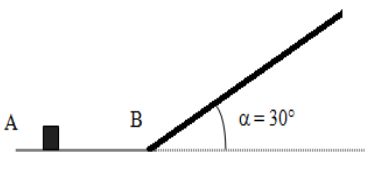
\includegraphics[width=0.38\textwidth]{./img/img00.png}
  \end{center}
\end{wrapfigure}
   Un autoporteur de masse $m = 600g$ est lancé depuis un point A avec une vitesse initiale $V_A = 6 m.s^{-1}$ sur un plan AB horizontal de longueur AB = 3 m sur lequel il glisse sans frottement, puis aborde un plan incliné BD , de
longueur $BD = 4 m$, sur lequel les frottements seront supposés négligeables.

L’autoporteur pourra être considéré comme un solide ponctuel. On prendra g = 10 N/Kg

1. Exprimer, puis calculer l’énergie cinétique de l’autoporteur en A.

2. Faire l’inventaire des forces extérieures agissant sur l’autoporteur au cours de la phase AB. Définir ces forces et les représenter sur un dessin

3.a. Donner la définition d’un système pseudo-isolé .

3.b. L’autoporteur est -il pseudo-isolé au cours de la phase AB et la phase BD ?

3.c. En déduire la vitesse du centre d’inertie du mobile en B ?

4. Soit $C_1$ un point du plan incliné tel que $BC_1 = 1 m$ Calculer le travail du poids de l’autoporteur et le travail de l’action du plan sur l’autoporteur au cours du
déplacement $BC_1$ .

   5. En appliquant le théorème de l’énergie cinétique au solide entre les instants $t_B$ et $t_{C_1}$ en déduire $V_{c_1}$

   6. Soit $C_2$ le point de rebroussement sur le plan incliné. En appliquant le théorème de l’énergie cinétique au solide entre les instants $t_B$ et $t_{C_2}$ , en déduire $BC_2$ la distance parcourue par le mobile avant de rebrousser chemin en $C_2$ .
\end{Box2}

%%_________________________Exercice 4 : _________________________Exercice
\begin{Box2}{Exercice 4 : }
Un corps solide, descend une pente
AB = 10 m en ligne droite, sans frottement,
le plan incliné fait angle $\alpha$ avec l’horizontale.
Au point A sa vitesse était nulle, à l’arrivée au point B sa vitesse est $V= 8 km.h^{-1}$ .
Calculer l’angle $\alpha$.
\end{Box2}
\vspace{2cm}
\begin{center}
   \Large{ \em{Exercices Supplémentaires}}
\end{center}



%%_________________________Exercice 5 : _________________________Exercice
\begin{Box2}{Exercice 5 : }
Un skieur de masse m = 100 kg (équipement compris) est tiré par un bateau à l'aide d'une corde parallèle à la surface de l'eau. 
\begin{center}
    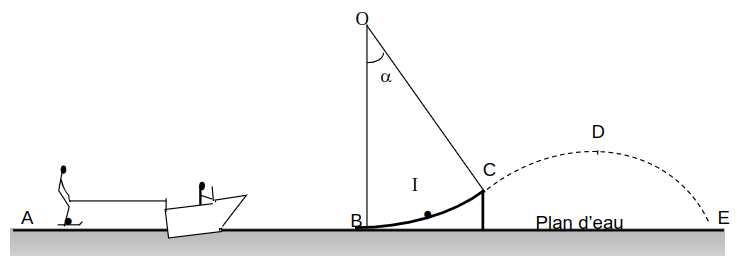
\includegraphics[width=1\textwidth, height =0.2\textwidth ]{./img/img01.png}
  \end{center}
Dans tout le problème, par souci de simplification on représentera les forces appliquéesau système \{skieur + skis\}  au niveau des skis

Données :$g = 10 N.kg^{-1}$ , $L = AB = 200 m$ ,  $\alpha=$30° ,  $OB = OC = 15 m$

   \underline{ \textbf{ $1^{\grave{e}re}$ étape (trajet AB): } } Le skieur démarre sans vitesse initiale du point A. Il est tracté par la force $\vec{F}$ constante et l’ensemble des forces de frottement est représenté par la force $\vec{f}$ d’intensité 100 N.Après un parcours de 200 m, le skieur atteint une vitesse $v_B= 20 m.s^{-1}$. 
\vspace{0.3cm}
\\1. Faire le bilan des forces s’exerçant sur le système \{skieur+skis\} sur la partie $A_B$.

2. Enoncé le théorème de l’énergie cinétique.

3. Exprimer les travaux des forces s’exerçant sur le système sur le trajet AB.

4. En déduire l’expressionla force de traction $\vec{F}$ en fonction de m, L, f, $v_B$.

5. Faire l’application numérique

\vspace{0.2cm}

   \underline{  \textbf{ $2^{\grave{e}me}$ étape (trajet BC):}} Le skieur lâche la corde en B et parcourt le tremplin BC qui est circulairede centre O de rayon OB = 15 m. OC fait un angle de 30° avec la verticale.Le tremplin est considéré comme parfaitement glissant.

\vspace{0.2cm}
6. Représenter sur le schéma au point I, les forces s’exerçant sur le système entre les points B et C (leurs caractéristiques ne sont pas demandées).

7. Exprimer la hauteur h acquise en haut du tremplin enfonction de OB et $\alpha$.

8. En appliquant le théorème de l’énergie cinétique, exprimer la vitesse $v_C$du skieur au point C en fonction de $v_B$, $\alpha$, g et OB.

9.Faire l’application numérique.

\vspace{0.2cm}
   \underline{  \textbf{ $3^{\grave{e}me}$ étape (trajet CE):}}Le skieur effectue un saut et retombe sur ses skis au point Ei Sur ce trajet, on supposera comme négligeable les frottements de l’air . La vitesse du skieur au point C est:  $v_C= 19 m.s^{-1}$ On prendra l’origine des altitudes en A.

10. Calculer l’énergie potentielle de pesanteur et l’énergie cinétique au point C.

11. La somme $E_c$ + $E_p$ est-elle constante entre C et E ? Justifier.

12. Représenter sur un graphique les variations des énergies cinétique et potentielle de pesanteur du skieur en fonction du temps sur le trajet CE. Justifier soigneusement l’allure des deux courbes.

13. La valeur de la vitesse au point D n’est pas nulle, elle vaut $v_D= 14 m.s^{-1}$.En utilisant la conservation de l’énergie totale du système, en déduire la hauteur du point D au dessus du plan d’eau en fonction des données de l’énoncé, puis calculer sa valeur.

14.En cas de frottements de l’air, que se passera-t-il en terme d’énergie et quelles peuvent être les conséquences sur le système?
\end{Box2}
%%_________________________Exercice 6 : _________________________Exercice
\end{document}
